\documentclass[11pt,a4paper]{article}
\usepackage[margin=2.2cm]{geometry}
\usepackage{tikz}
\usepackage{booktabs}
\usepackage{array}
\usepackage{float}
\usepackage{graphicx}
\usetikzlibrary{arrows.meta,positioning,calc}

\title{Cyber Physical Robotics: Milestone 2\\
       \large Distributed Robot Control with Ideal Communication}
\author{}
\date{}

\begin{document}
\maketitle
\vspace{-2.5em}

\section{Approach}
Targets must be picked up by exactly two robots at the same time. There is no
central controller. Every robot runs the same state machine and decides for
itself, using only what it senses and the messages it reads. Communication is
ideal: a message broadcast at the end of one step is read by every other robot
at the start of the next step.

\section{Messages}
\begin{tabular}{@{}lp{11.2cm}@{}}
\toprule
\textbf{Message} & \textbf{Content and purpose}\\
\midrule
\texttt{FOUND} & Goal id, goal position, sender id. Sent by a robot that senses a goal in front of it.\\
\texttt{POS}   & Goal id, sender id, sender position. Sent by every free robot that reads a \texttt{FOUND}.\\
\texttt{READY} & Goal id, sender id, partner id. Sent while the partner is on the sender's cell.\\
\texttt{PICKED} & Goal id, sender id. Sent when a robot picks up, so others drop that goal.\\
\bottomrule
\end{tabular}

\section{State machine}
\begin{figure}[H]
\centering
\resizebox{\linewidth}{!}{%
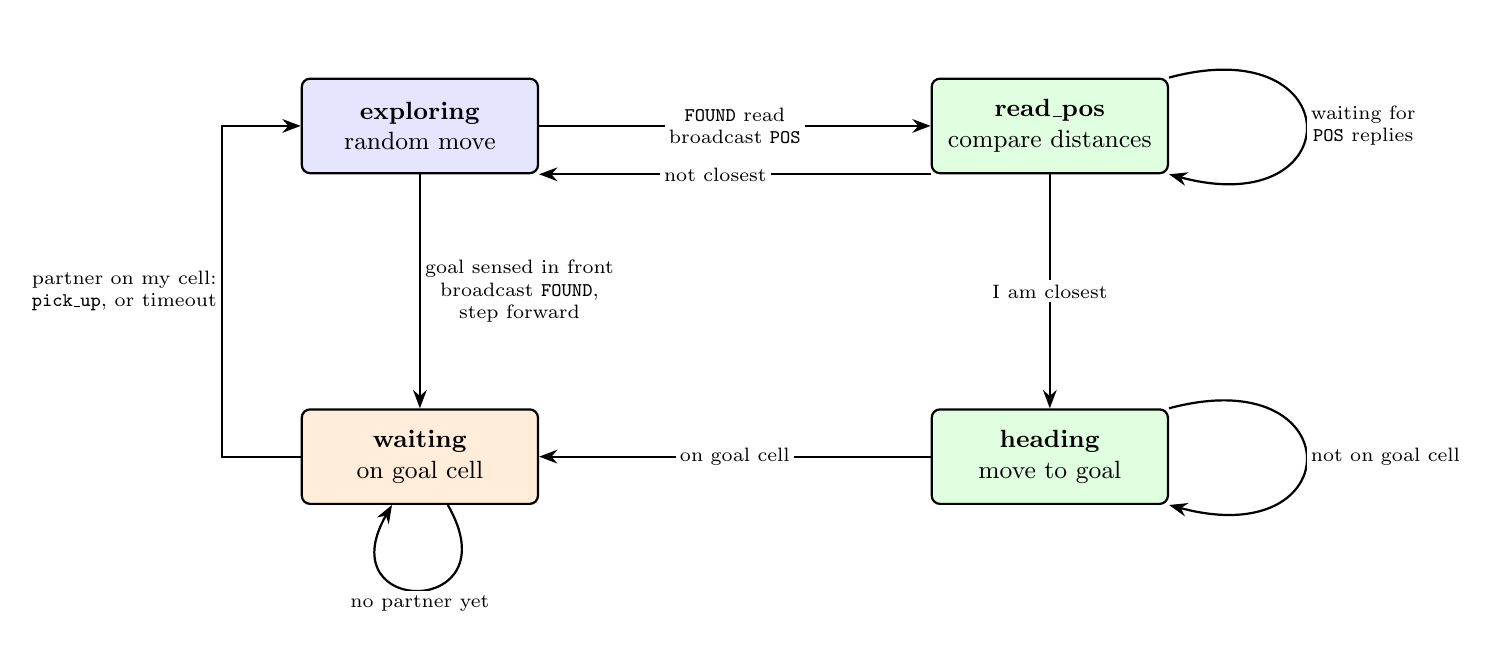
\begin{tikzpicture}[
    >=Stealth, thick,
    state/.style={draw, rounded corners=3pt, minimum width=3cm,
                  minimum height=1.2cm, align=center, font=\small},
    lbl/.style={font=\scriptsize, align=center, fill=white, inner sep=1.5pt}
]
\node[state, fill=blue!10]   (explore) at (0,0)   {\textbf{exploring}\\random move};
\node[state, fill=orange!15] (wait)    at (0,-4.2)  {\textbf{waiting}\\on goal cell};
\node[state, fill=green!12]  (readpos) at (8,0)   {\textbf{read\_pos}\\compare distances};
\node[state, fill=green!12]  (head)    at (8,-4.2)  {\textbf{heading}\\move to goal};

% finder
\draw[->] (explore.south) -- node[lbl, right, pos=.5]{goal sensed in front\\
  broadcast \texttt{FOUND},\\step forward} (wait.north);
% helper
\draw[->] (explore.east) -- node[lbl, pos=.5]{\texttt{FOUND} read\\broadcast \texttt{POS}} (readpos.west);
\draw[->] (readpos.south) -- node[lbl, pos=.5]{I am closest} (head.north);
\draw[->] (readpos.south west) -- node[lbl, pos=.55]{not closest} (explore.south east);
\draw[->] (head.west) -- node[lbl, pos=.5]{on goal cell} (wait.east);
% back to exploring after pick
\draw[->] (wait.west) -- ++(-1.0,0) |- node[lbl, pos=.25, left]{partner on my cell:\\
  \texttt{pick\_up}, or timeout} (explore.west);
% loops
\draw[->] (readpos.north east) to[loop right, looseness=5] node[lbl, right]{waiting for\\\texttt{POS} replies} (readpos.south east);
\draw[->] (head.north east) to[loop right, looseness=5] node[lbl, right]{not on goal cell} (head.south east);
\draw[->] (wait.-60) to[out=-60, in=-120, looseness=6] node[lbl, below]{no partner yet} (wait.-120);
\end{tikzpicture}}
\caption{State machine run by every robot.}
\end{figure}

\section{State descriptions}
\begin{description}
\item[exploring] The robot moves randomly (forward, turn left, turn right) and
never picks up. If it reads a \texttt{FOUND}, it broadcasts its own position in
a \texttt{POS} and goes to \emph{read\_pos}; if several goals were announced it
takes the lowest goal id. Otherwise, if it senses a goal directly in front, it
broadcasts \texttt{FOUND}, steps onto the goal and goes to \emph{waiting}.

\item[read\_pos] The robot collects the \texttt{POS} messages for its goal.
Each robot ranks all positions, including its own, by Manhattan distance to the
goal, with the lowest id breaking ties. All robots see the same replies, so they
agree on the winner. The finder is already on the goal, so exactly one more
robot is needed: the closest robot goes to \emph{heading}, the others return to
\emph{exploring}.

\item[heading] The robot turns and moves toward the goal cell, fixing the
x~coordinate first and then y. On arrival it goes to \emph{waiting}.

\item[waiting] The robot stands on the goal cell and stays idle. Its partner is
known by id: the helper's partner is the finder, and the finder's partner is the
closest robot that answered with \texttt{POS} (or the other finder, if two robots
found the goal at once). While the partner is sensed on its cell, the robot
broadcasts \texttt{READY}. It picks only after it has sent \texttt{READY} and
read the partner's \texttt{READY}, which names it as partner. Both robots then
perform \texttt{pick\_up} in the same step, broadcast \texttt{PICKED} and return
to \emph{exploring}. A robot also returns to \emph{exploring} when it reads
\texttt{PICKED} for its goal, or when no partner comes within a fixed number of
steps.
\end{description}

\section{Why picks are legal}
Being on the goal cell is not enough, because the partner may still be
deciding. A robot therefore picks only when its partner is on the cell and the
two robots have agreed through \texttt{READY}, each naming the other. Pairs must
agree, so a robot never picks with a partner that has chosen someone else.
Robots also remember goals that were already announced and do not announce them
again, so a goal does not collect several pairs. In simulation (100 runs of 2500
steps, 2 to 15 robots) this gave no illegal pick in about 9500 successful picks.

\end{document}
